% The same refutation, regenerated by the trusted kernel: five variables, ten clauses.
% Build: pdflatex sat_evidence_check.tex
\documentclass[tikz,border=3pt]{standalone}
\usepackage{lmodern,amsmath,amssymb}
\usetikzlibrary{arrows.meta,calc}
\begin{document}
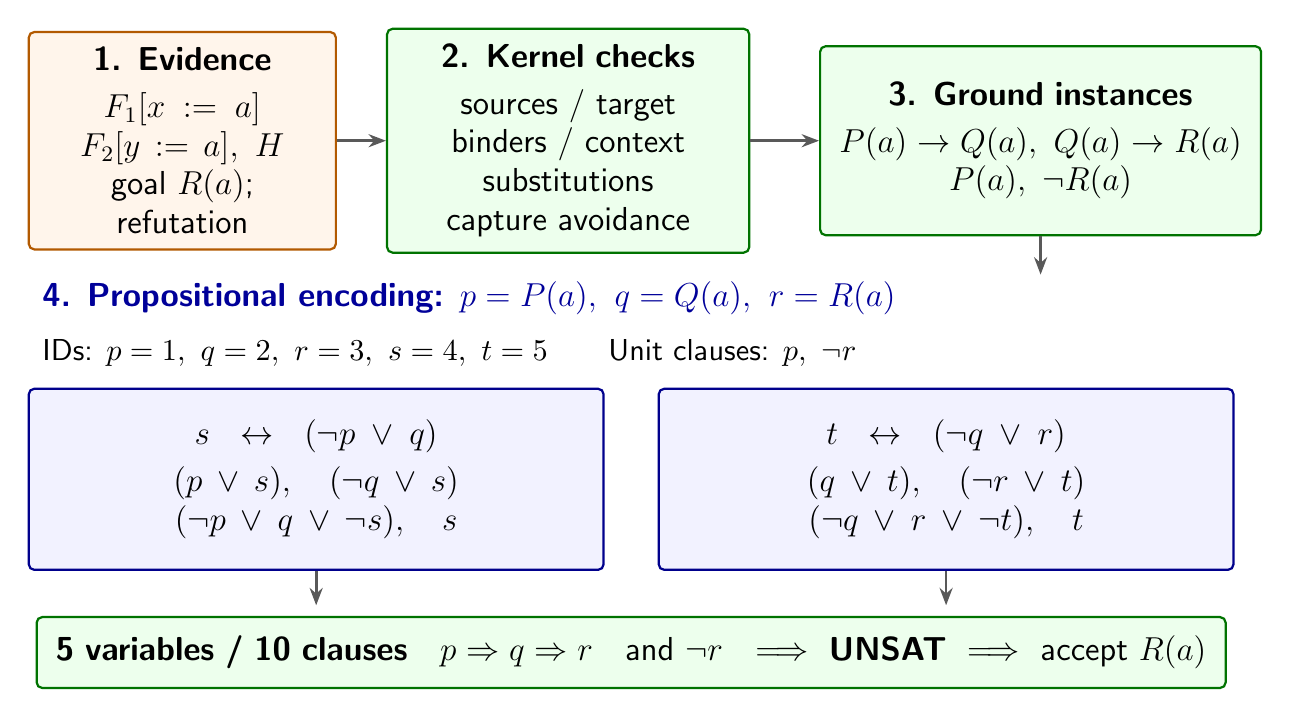
\begin{tikzpicture}[
  font=\sffamily\fontsize{12}{14}\selectfont,
  box/.style={draw,rounded corners=2pt,line width=.8pt,align=center,inner sep=2mm},
  input/.style={box,draw=orange!70!black,fill=orange!8},
  kernel/.style={box,draw=green!45!black,fill=green!7},
  cnf/.style={box,draw=blue!55!black,fill=blue!5},
  flow/.style={-{Stealth[length=2.2mm]},line width=1pt,black!65},
  head/.style={font=\sffamily\bfseries\fontsize{13}{15}\selectfont},
]
\node[input,text width=35mm,minimum height=24mm] (e) at (18mm,0)
  {\textbf{1. Evidence}\\[1mm]
   $F_1[x:=a]$\\
   $F_2[y:=a],\ H$\\
   goal $R(a)$; refutation};
\node[kernel,text width=42mm,minimum height=24mm] (k) at (67mm,0)
  {\textbf{2. Kernel checks}\\[1mm]
   sources / target\\
   binders / context\\
   substitutions\\
   capture avoidance};
\node[kernel,text width=52mm,minimum height=24mm] (i) at (127mm,0)
  {\textbf{3. Ground instances}\\[1mm]
   $P(a)\to Q(a),\ Q(a)\to R(a)$\\
   $P(a),\ \neg R(a)$};
\draw[flow] (e) -- (k);
\draw[flow] (k) -- (i);
\node[head,anchor=west,text=blue!60!black] at (-1mm,-20mm)
  {4. Propositional encoding: $p=P(a),\ q=Q(a),\ r=R(a)$};
\node[anchor=west,font=\sffamily\fontsize{11}{13}\selectfont] at (-1mm,-27mm)
  {IDs: $p=1,\ q=2,\ r=3,\ s=4,\ t=5$\qquad Unit clauses: $p,\ \neg r$};
\node[cnf,text width=69mm,minimum height=23mm] (s) at (35mm,-43mm)
  {$s\leftrightarrow(\neg p\lor q)$\\[1mm]
   $(p\lor s),\quad(\neg q\lor s)$\\
   $(\neg p\lor q\lor\neg s),\quad s$};
\node[cnf,text width=69mm,minimum height=23mm] (t) at (115mm,-43mm)
  {$t\leftrightarrow(\neg q\lor r)$\\[1mm]
   $(q\lor t),\quad(\neg r\lor t)$\\
   $(\neg q\lor r\lor\neg t),\quad t$};
\draw[flow] (i.south) -- (127mm,-17mm);
\node[kernel,text width=147mm,minimum height=9mm] at (75mm,-65mm)
  {\textbf{5 variables / 10 clauses}\quad
   $p\Rightarrow q\Rightarrow r$\quad and $\neg r$\quad
   $\Longrightarrow\ \textbf{UNSAT}\ \Longrightarrow\ \text{accept }R(a)$};
\draw[flow] (s.south) -- (35mm,-59mm);
\draw[flow] (t.south) -- (115mm,-59mm);
\end{tikzpicture}
\end{document}
